\documentclass[journal,12pt,twocolumn]{IEEEtran}
%
\usepackage{setspace}
\usepackage{gensymb}
\usepackage{xcolor}
\usepackage{caption}
\usepackage{polynom}
%\usepackage{subcaption}
%\doublespacing
\singlespacing

%\usepackage{graphicx}
%\usepackage{amssymb}
%\usepackage{relsize}
\usepackage[cmex10]{amsmath}
\usepackage{mathtools}
%\usepackage{amsthm}
%\interdisplaylinepenalty=2500
%\savesymbol{iint}
%\usepackage{txfonts}
%\restoresymbol{TXF}{iint}
%\usepackage{wasysym}
\usepackage{hyperref}
\usepackage{amsthm}
\usepackage{mathrsfs}
\usepackage{txfonts}
\usepackage{stfloats}
\usepackage{cite}
\usepackage{cases}
\usepackage{subfig}
%\usepackage{xtab}
\usepackage{longtable}
\usepackage{multirow}
%\usepackage{algorithm}
%\usepackage{algpseudocode}
%\usepackage{enumerate}
\usepackage{enumitem}
\usepackage{mathtools}
%\usepackage{iithtlc}
%\usepackage[framemethod=tikz]{mdframed}
\usepackage{listings}
\usepackage{polynom}

%\usepackage{stmaryrd}


%\usepackage{wasysym}
%\newcounter{MYtempeqncnt}
\DeclareMathOperator*{\Res}{Res}
%\renewcommand{\baselinestretch}{2}
\renewcommand\thesection{\arabic{section}}
\renewcommand\thesubsection{\thesection.\arabic{subsection}}
\renewcommand\thesubsubsection{\thesubsection.\arabic{subsubsection}}

\renewcommand\thesectiondis{\arabic{section}}
\renewcommand\thesubsectiondis{\thesectiondis.\arabic{subsection}}
\renewcommand\thesubsubsectiondis{\thesubsectiondis.\arabic{subsubsection}}

%\renewcommand{\labelenumi}{\textbf{\theenumi}}
%\renewcommand{\theenumi}{P.\arabic{enumi}}

% correct bad hyphenation here
\hyphenation{op-tical net-works semi-conduc-tor}

\makeatletter
\def\pld@CF@loop#1+{%
    \ifx\relax#1\else
        \begingroup
          \pld@AccuSetX11%
          \def\pld@frac{{}{}}\let\pld@symbols\@empty\let\pld@vars\@empty
          \pld@false
          #1%
          \let\pld@temp\@empty
          \pld@AccuIfOne{}{\pld@AccuGet\pld@temp
                            \edef\pld@temp{\noexpand\pld@R\pld@temp}}%
           \pld@if \pld@Extend\pld@temp{\expandafter\pld@F\pld@frac}\fi
           \expandafter\pld@CF@loop@\pld@symbols\relax\@empty
           \expandafter\pld@CF@loop@\pld@vars\relax\@empty
           \ifx\@empty\pld@temp
               \def\pld@temp{\pld@R11}%
           \fi
          \global\let\@gtempa\pld@temp
        \endgroup
        \ifx\@empty\@gtempa\else
            \pld@ExtendPoly\pld@tempoly\@gtempa
        \fi
        \expandafter\pld@CF@loop
    \fi}
\def\pld@CMAddToTempoly{%
    \pld@AccuGet\pld@temp\edef\pld@temp{\noexpand\pld@R\pld@temp}%
    \pld@CondenseMonomials\pld@false\pld@symbols
    \ifx\pld@symbols\@empty \else
        \pld@ExtendPoly\pld@temp\pld@symbols
    \fi
    \ifx\pld@temp\@empty \else
        \pld@if
            \expandafter\pld@IfSum\expandafter{\pld@temp}%
                {\expandafter\def\expandafter\pld@temp\expandafter
                    {\expandafter\pld@F\expandafter{\pld@temp}{}}}%
                {}%
        \fi
        \pld@ExtendPoly\pld@tempoly\pld@temp
        \pld@Extend\pld@tempoly{\pld@monom}%
    \fi}
\makeatother

\lstset{
language=Python,
frame=single, 
breaklines=true,
columns=fullflexible
}



\begin{document}
%

\theoremstyle{definition}
\newtheorem{theorem}{Theorem}[section]
\newtheorem{problem}{Problem}
\newtheorem{proposition}{Proposition}[section]
\newtheorem{lemma}{Lemma}[section]
\newtheorem{corollary}[theorem]{Corollary}
\newtheorem{example}{Example}[section]
\newtheorem{definition}{Definition}[section]
%\newtheorem{algorithm}{Algorithm}[section]
%\newtheorem{cor}{Corollary}
\newcommand{\BEQA}{\begin{eqnarray}}
\newcommand{\EEQA}{\end{eqnarray}}
\newcommand{\define}{\stackrel{\triangle}{=}}
\bibliographystyle{IEEEtran}
%\bibliographystyle{ieeetr}
\providecommand{\nCr}[2]{\,^{#1}C_{#2}} % nCr
\providecommand{\nPr}[2]{\,^{#1}P_{#2}} % nPr
\providecommand{\mbf}{\mathbf}
\providecommand{\pr}[1]{\ensuremath{\Pr\left(#1\right)}}
\providecommand{\qfunc}[1]{\ensuremath{Q\left(#1\right)}}
\providecommand{\sbrak}[1]{\ensuremath{{}\left[#1\right]}}
\providecommand{\lsbrak}[1]{\ensuremath{{}\left[#1\right.}}
\providecommand{\rsbrak}[1]{\ensuremath{{}\left.#1\right]}}
\providecommand{\brak}[1]{\ensuremath{\left(#1\right)}}
\providecommand{\lbrak}[1]{\ensuremath{\left(#1\right.}}
\providecommand{\rbrak}[1]{\ensuremath{\left.#1\right)}}
\providecommand{\cbrak}[1]{\ensuremath{\left\{#1\right\}}}
\providecommand{\lcbrak}[1]{\ensuremath{\left\{#1\right.}}
\providecommand{\rcbrak}[1]{\ensuremath{\left.#1\right\}}}
\theoremstyle{remark}
\newtheorem{rem}{Remark}
\newcommand{\sgn}{\mathop{\mathrm{sgn}}}
\providecommand{\abs}[1]{\left\vert#1\right\vert}
\providecommand{\res}[1]{\Res\displaylimits_{#1}} 
\providecommand{\norm}[1]{\lVert#1\rVert}
\providecommand{\mtx}[1]{\mathbf{#1}}
\providecommand{\mean}[1]{E\left[ #1 \right]}
\providecommand{\fourier}{\overset{\mathcal{F}}{ \rightleftharpoons}}
\providecommand{\ztrans}{\overset{\mathcal{Z}}{ \rightleftharpoons}}
%\providecommand{\hilbert}{\overset{\mathcal{H}}{ \rightleftharpoons}}
\providecommand{\system}{\overset{\mathcal{H}}{ \longleftrightarrow}}
	%\newcommand{\solution}[2]{\textbf{Solution:}{#1}}
	\newcommand{\myvec}[1]{\ensuremath{\begin{pmatrix}#1\end{pmatrix}}}
	\newcommand{\mybvec}[1]{\ensuremath{\begin{bmatrix}#1\end{bmatrix}}}
	\newcommand{\w}[2]{\ensuremath{W_{#1}^{#2}}}
\newcommand{\solution}{\noindent \textbf{Solution: }}
\providecommand{\dec}[2]{\ensuremath{\overset{#1}{\underset{#2}{\gtrless}}}}
\numberwithin{equation}{section}
%\numberwithin{equation}{subsection}
%\numberwithin{problem}{subsection}
%\numberwithin{definition}{subsection}
\renewcommand{\thefigure}{\theproblem.\arabic{figure}}
\let\vec\mathbf
\makeatletter
\@addtoreset{figure}{problem}
\makeatother
\let\StandardTheFigure\thefigure
% \renewcommand{\thefigure}{\theproblem}
%\numberwithin{figure}{subsection}
\def\putbox#1#2#3{\makebox[0in][l]{\makebox[#1][l]{}\raisebox{\baselineskip}[0in][0in]{\raisebox{#2}[0in][0in]{#3}}}}
     \def\rightbox#1{\makebox[0in][r]{#1}}
     \def\centbox#1{\makebox[0in]{#1}}
     \def\topbox#1{\raisebox{-\baselineskip}[0in][0in]{#1}}
     \def\midbox#1{\raisebox{-0.5\baselineskip}[0in][0in]{#1}}
\vspace{3cm}
\title{ 
%\logo{
Digital Signal Processing 
%}
%	\logo{Octave for Math Computing }
}
%\title{
%	\logo{Matrix Analysis through Octave}{\begin{center}\includegraphics[scale=.24]{tlc}\end{center}}{}{HAMDSP}
%}
% paper title
% can use linebreaks \\ within to get better formatting as desired
%\title{Matrix Analysis through Octave}
%
%
% author names and IEEE memberships
% note positions of commas and nonbreaking spaces ( ~ ) LaTeX will not break
% a structure at a ~ so this keeps an author's name from being broken across
% two lines.
% use \thanks{} to gain access to the first footnote area
% a separate \thanks must be used for each paragraph as LaTeX2e's \thanks
% was not built to handle multiple paragraphs
%
\author{ Ameya Chatur \\BM20BTECH11002%<-this  stops a space
%\thanks{*The author is with the Department
%of Electrical Engineering, Indian Institute of Technology, Hyderabad
%502285 India e-mail:  gadepall@iith.ac.in.  All content in the manuscript is 
%released under GNU GPL.  Free to use for anything. }% <-this % stops a space
%\thanks{J. Doe and J. Doe are with Anonymous University.}% <-this % stops a space
%\thanks{Manuscript received April 19, 2005; revised January 11, 2007.}}
}
% note the % following the last \IEEEmembership and also \thanks - 
% these prevent an unwanted space from occurring between the last author name
% and the end of the author line. i.e., if you had this:
% 
% \author{....lastname \thanks{...} \thanks{...} }
%                     ^------------^------------^----Do not want these spaces!
%
% a space would be appended to the last name and could cause every name on that
% line to be shifted left slightly. This is one of those "LaTeX things". For
% instance, "\textbf{A} \textbf{B}" will typeset as "A B" not "AB". To get
% "AB" then you have to do: "\textbf{A}\textbf{B}"
% \thanks is no different in this regard, so shield the last } of each \thanks
% that ends a line with a % and do not let a space in before the next \thanks.
% Spaces after \IEEEmembership other than the last one are OK (and needed) as
% you are supposed to have spaces between the names. For what it is worth,
% this is a minor point as most people would not even notice if the said evil
% space somehow managed to creep in.
% The paper headers
%\markboth{Journal of \LaTeX\ Class Files,~Vol.~6, No.~1, January~2007}%
%{Shell \MakeLowercase{\textit{et al.}}: Bare Demo of IEEEtran.cls for Journals}
% The only time the second header will appear is for the odd numbered pages
% after the title page when using the twoside option.
% 
% *** Note that you probably will NOT want to include the author's ***
% *** name in the headers of peer review papers.                   ***
% You can use \ifCLASSOPTIONpeerreview for conditional compilation here if
% you desire.
% If you want to put a publisher's ID mark on the page you can do it like
% this:
%\IEEEpubid{0000--0000/00\$00.00~\copyright~2007 IEEE}
% Remember, if you use this you must call \IEEEpubidadjcol in the second
% column for its text to clear the IEEEpubid mark.
% make the title area
\maketitle
%\newpage
\tableofcontents
%\renewcommand{\thefigure}{\thesection.\theenumi}
%\renewcommand{\thetable}{\thesection.\theenumi}
\renewcommand{\thefigure}{\theenumi}
\renewcommand{\thetable}{\theenumi}
%\renewcommand{\theequation}{\thesection}
\bigskip
\begin{abstract}
This manual provides a simple introduction to digital signal processing.
\end{abstract}
\section{Software Installation}
Run the following commands
\begin{lstlisting}
sudo apt-get update
sudo apt-get install libffi-dev libsndfile1 python3-scipy  python3-numpy python3-matplotlib 
sudo pip install cffi pysoundfile 
\end{lstlisting}
\section{Digital Filter}
\begin{enumerate}[label=\thesection.\arabic*
,ref=\thesection.\theenumi]
\item
\label{prob:input}
Download the sound file from  
\begin{lstlisting}
wget https://github.com/yashrajput22/EE3900-22/blob/master/codes/Section-2/Sound_Noise.wav
\end{lstlisting}
%\href{http://tlc.iith.ac.in/img/sound/Sound_Noise.wav}{\url{http://tlc.iith.ac.in/img/sound/Sound_Noise.wav}}  
%in the link given below.
%\linebreak
\item
\label{prob:spectrogram}
You will find a spectrogram at \href{https://academo.org/demos/spectrum-analyzer}{\url{https://academo.org/demos/spectrum-analyzer}}. 
%\end{problem}
%%
%
%%\onecolumn
%%\input{./figs/fir}
%\begin{problem}
Upload the sound file that you downloaded in Problem \ref{prob:input} in the spectrogram  and play.  Observe the spectrogram. What do you find?
\\
%
\solution There are a lot of yellow lines between 440 Hz to 5.1 KHz.  These represent the synthesizer key tones. Also, the key strokes
are audible along with background noise.
% By observing spectrogram, it clearly shows that tonal frequency is under 4kHz. And above 4kHz only noise is present.
\item
\label{prob:output}
Write the python code for removal of out of band noise and execute the code.
\\
\solution
\lstinputlisting{codes/2_3.py}
\item
The output of the python script in Problem \ref{prob:output} is the audio file Sound\_With\_ReducedNoise.wav. Play the file in the spectrogram in Problem \ref{prob:spectrogram}. What do you observe?
\\
\solution The key strokes as well as background noise is subdued in the audio.  Also,  the signal is blank for frequencies above 5.1 kHz.
\end{enumerate}
\section{Difference Equation}
\begin{enumerate}[label=\thesection.\arabic*,ref=\thesection.\theenumi]
\item Let
 \label{def:xn}
\begin{equation}
x(n) = \cbrak{\underset{\uparrow}{1},2,3,4,2,1}
\end{equation}
Sketch $x(n)$.
\\
\solution
\lstinputlisting{codes/3_1.py}
\text{The above code yields}
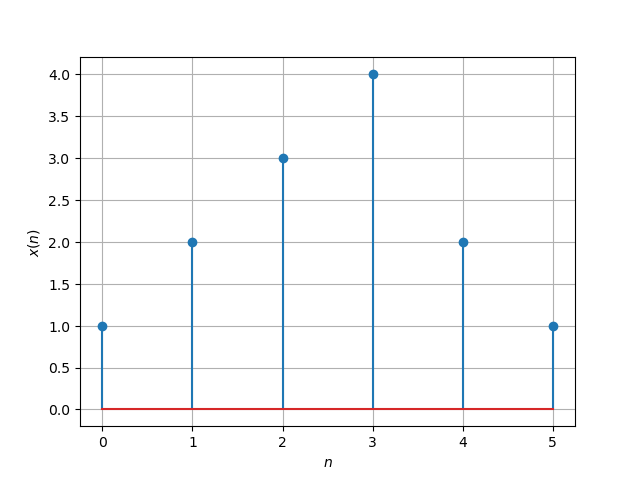
\includegraphics[width=\columnwidth]{figures/Figure_3_1.png}
\item Let
\begin{multline}
\label{eq:iir_filter}
y(n) + \frac{1}{2}y(n-1) = x(n) + x(n-2),
\\
 y(n) = 0, n < 0
\end{multline}
Sketch $y(n)$.  
\\
\solution 
\lstinputlisting{codes/3_2.py}
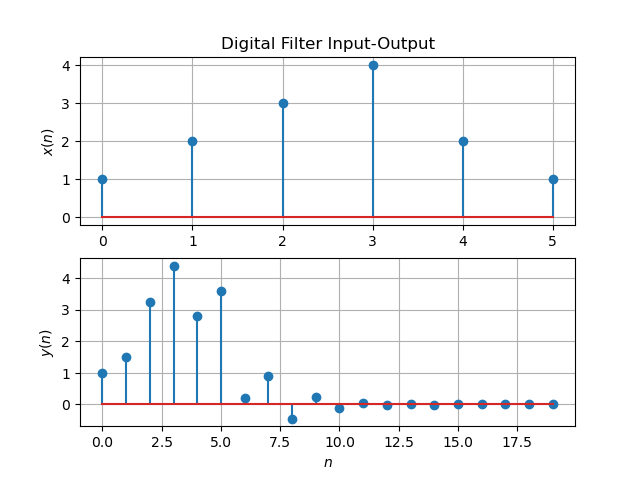
\includegraphics[width=\columnwidth]{figures/Figure_3_2.png}

\item Repeat the above exercise using a C code.
\\
\solution
The following C code generates data and saves it to a .dat file
\lstinputlisting{codes/3_3.c}
The following Python code sketches $x(n)$ and $y(n)$
\lstinputlisting{codes/3_3.py}
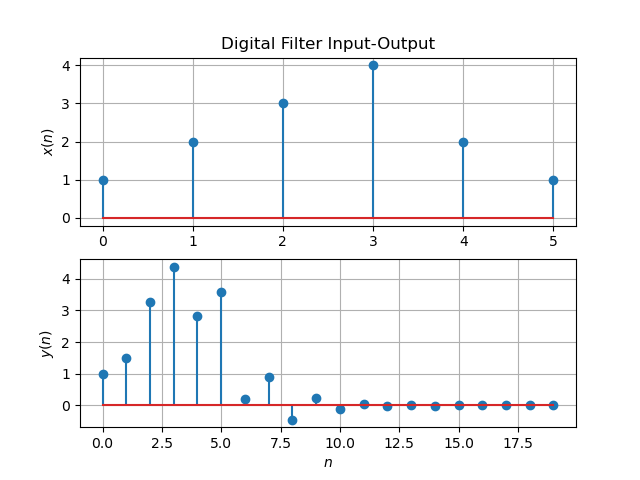
\includegraphics[width=\columnwidth]{figures/Figure_3_3.png}
\end{enumerate}

\section{$Z$-transform}
\begin{enumerate}[label=\thesection.\arabic*]
\item The $Z$-transform of $x(n)$ is defined as
%
\begin{equation}
\label{z_trans}
X(z)={\mathcal {Z}}\{x(n)\}=\sum _{n=-\infty }^{\infty }x(n)z^{-n}
\end{equation}
%
Show that
\begin{equation}
\label{eq:shift1}
{\mathcal {Z}}\{x(n-1)\} = z^{-1}X(z)
\end{equation}
and find
\begin{equation}
	{\mathcal {Z}}\{x(n-k)\} 
\end{equation}
\solution From \eqref{eq:z_trans},
\begin{align}
{\mathcal {Z}}\{x(n-1)\} &=\sum _{n=-\infty }^{\infty }x(n-1)z^{-n}
\\
&=\sum _{n=-\infty }^{\infty }x(n)z^{-n-1} = z^{-1}\sum _{n=-\infty }^{\infty }x(n)z^{-n}
\end{align}
resulting in \eqref{eq:shift1}. Similarly, it can be shown that
%
\begin{equation}
\label{eq:z_trans_shift}
	{\mathcal {Z}}\{x(n-k)\} = z^{-k}X(z)
\end{equation}
\item Obtain $X(z)$ for $x(n)$ defined in problem  \ref{def:xn}.
\solution
\begin{align}
Z(x(n))&=\sum_{n=-\infty}^{\infty}x(n)z^{-n}\\
&=x(0)z^{0}+x(1)z^{-1}+x(2)z^{-2}+x(3)z^{-3}+\\
&\nonumber x(4)z^{-4}+x(5)z^{-5}\\
&=1+2z^{-1}+3z^{-2}+4z^{-3}+2z^{-4}+z^{-5}
\end{align}
\item Find
%
\begin{equation}
H(z) = \frac{Y(z)}{X(z)}
\end{equation}
%
from  \eqref{eq:iir_filter} assuming that the $Z$-transform is a linear operation.
\\
\solution 
\\
Applying \eqref{eq:z_trans_shift} in \eqref{eq:iir_filter},
\begin{align}
Y(z) + \frac{1}{2}z^{-1}Y(z) &= X(z)+z^{-2}X(z)
\\
\implies \frac{Y(z)}{X(z)} &= \frac{1 + z^{-2}}{1 + \frac{1}{2}z^{-1}}
\label{eq:freq_resp}
\end{align}
%
\item Find the Z transform of 
\begin{equation}
\delta(n)
=
\begin{cases}
1 & n = 0
\\
0 & \text{otherwise}
\end{cases}
\end{equation}
and show that the $Z$-transform of
\begin{equation}
\label{eq:unit_step}
u(n)
=
\begin{cases}
1 & n \ge 0
\\
0 & \text{otherwise}
\end{cases}
\end{equation}
is
\begin{equation}
U(z) = \frac{1}{1-z^{-1}}, \quad \abs{z} > 1
\end{equation}
\solution It is easy to show that
\begin{equation}
\delta(n) \ztrans 1
\end{equation}
and from \eqref{eq:unit_step},
\begin{align}
U(z) &= \sum _{n= 0}^{\infty}z^{-n}
\\
&=\frac{1}{1-z^{-1}}, \quad \abs{z} > 1
\end{align}
using the fomula for the sum of an infinite geometric progression.
%
\item Show that 
\begin{equation}
\label{eq:anun}
a^nu(n) \ztrans \frac{1}{1-az^{-1}} \quad \abs{z} > \abs{a}
\end{equation}
\solution
\begin{align}
{\mathcal {Z}}\{a^nu(n)\} &=\sum _{n=-\infty }^{\infty }a^nu(n)z^{-n}
\\
&=\sum _{n=-\infty }^{\infty }u(n) (az^{-1})^{n}
\\
&=\sum _{n=0 }^{\infty }(az^{-1})^{n} , \quad \abs{az^{-1}} < 1\\
\\
&= \frac{1}{1-az^{-1}} , \quad \abs{a} < \abs{z}
\end{align}
using the fomula for the sum of an infinite geometric progression.
%
\item 
Let
\begin{equation}
H\brak{e^{\j \omega}} = H\brak{z = e^{\j \omega}}.
\end{equation}
Plot $\abs{H\brak{e^{\j \omega}}}$.  Comment.  $H(e^{\j \omega})$ is
known as the {\em Discret Time Fourier Transform} (DTFT) of $x(n)$.
\\
\solution  The graph is symmetric and periodic. It is achieves a high of value 4 and a minimum value between 0 - 0.5. 
It is bounded between (0, 4) with period of $2\pi$
\\
\begin{align}
	H\brak{e^{j \omega}} &= \frac{1+e^{-2j\omega}}{1 + \frac{e^{-j\omega}}{2}}\\
	  \implies \abs{H\brak{e^{j \omega}}} &= \frac{\abs{1+e^{-2j\omega}}}{\abs{1 + \frac{e^{-j\omega}}{2}}}\\
						  &= \frac{\abs{1+e^{2j\omega}}}{\abs{e^{2j\omega} + \frac{e^{j\omega}}{2}}}\\
						  &= \frac{\abs{1+\cos2\omega + j\sin2\omega}}{\abs{e^{j\omega}+ \frac{1}{2}}}\\
						  &= \frac{\abs{4\cos^2\brak{\omega} + 4j\sin\brak{\omega}\cos\brak{\omega}}}{\abs{2e^{j\omega} + 1}}\\
						  &= \frac{\abs{4\cos\brak{\omega}}\abs{\cos\brak{\omega} + j\sin\brak{\omega}}}{\abs{2\cos\brak{\omega} + 1 + 2j\sin\brak{\omega}}}\\
	  \therefore \abs{H\brak{e^{j \omega}}} &= \frac{\abs{4\cos\brak{\omega}}}{\sqrt{5 +4\cos\brak{\omega}}}
\end{align}
The following code plots $\abs{H\brak{e^{j \omega}}}$
\lstinputlisting{codes/4_6.py}
\begin{figure}[!ht]
	\centering
	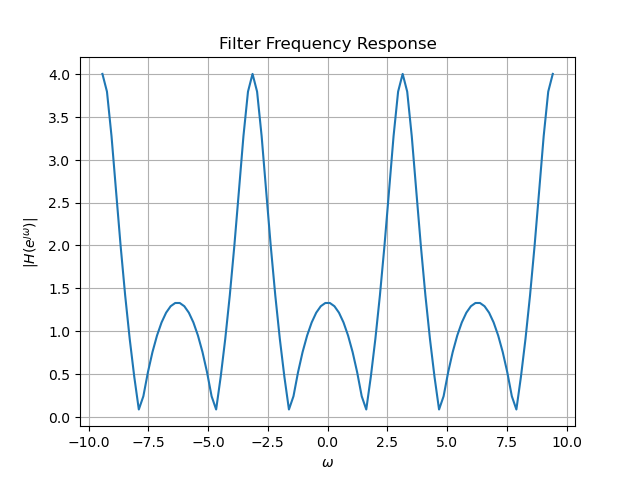
\includegraphics[width=\columnwidth]{figures/Figure_4_6.png}
	\caption{$h(n)$ as the inverse of $H(z)$}
	\end{figure}
\item Express $h(n)$ in terms of $H\brak{e^{\j \omega}}$.\\
\solution 
\begin{align}
	H\brak{e^{j\omega}} &= \sum_{n=-\infty}^{\infty} h\brak{n} e^{-j\omega n}
	\\
	\int_{-\pi}^{\pi}H\brak{e^{j\omega}}e^{j\omega k}d\omega &= \sum_{n=-\infty}^{\infty} h\brak{n} \int_{-\pi}^{\pi} e^{-j\omega n}e^{j\omega k}d\omega
	\\
	\\
		\int_{-\pi}^{\pi}e^{\j\omega(n - k)}d\omega &=
		\begin{cases}
			2\pi & n = k \\
			0 & \textrm{otherwise}
		\end{cases}
    \\
	\int_{-\pi}^{\pi}H\brak{e^{j\omega}}e^{j\omega k}d\omega &= h\brak{n} 2\pi
    \\
    \int_{-\pi}^{\pi}H\brak{e^{j\omega}}e^{j\omega k}d\omega &= 2\pi h\brak{n} 
	\\
	\frac{1}{2\pi} \int_{-\pi}^{\pi}H\brak{e^{j\omega}}e^{j\omega k}d\omega &= h\brak{n} 
\end{align} 
\end{enumerate}
\section{Impulse Response}
\begin{enumerate}[label=\thesection.\arabic*]
	\item Using long division, 
find
		\begin{align}
			h(n), \quad n < 5
		\end{align}
		for H(z) in 
		\eqref{eq:freq_resp}.
		\\\solution\\
		\begin{equation}
			H(z) = \frac{1 + z^{-2}}{1 + \frac{1}{2} z^{-1}}
		\end{equation}
		Let $z^{-1} = x$,then, by polynomial long division we get
		
		\polylongdiv{1+x^2}{1+\frac12 x}
	\begin{align}
		\implies (1+z^{-2})= (\frac{1}{2} z^{-1}+1)(2z^{-1}-4) + 5
		\\\implies \frac{(1+z^{-2})}{\frac{1}{2} z^{-1}+1}= (2z^{-1}-4) + \frac{5}{\frac{1}{2} z^{-1}+1}
		\\\implies H\brak{z}=(2z^{-1}-4) + \frac{5}{\frac{1}{2} z^{-1}+1}
	\end{align}
	Now, consider$ \frac{5}{\frac{1}{2} z^{-1}+1}$
	\\The denominator $\frac{1}{2} z^{-1}+1$ can be expressed as sum of an infinite geometric progression, which as its first term equal to 1 and common ratio $\frac{-1}{2}z^{-1}$
	\\Therefore, we can write $ \frac{5}{\frac{1}{2} z^{-1}+1}$ as 5\brak{1+\brak{\frac{-1}{2}z^{-1}}+\brak{\frac{-1}{2}z^{-1}}^{2}+\brak{\frac{-1}{2}z^{-1}}^{3}+\brak{\frac{-1}{2}z^{-1}}^{4}+\dots}	
	\\Therefore, H(z) can be given by,
	\\\begin{equation}
		H(z)= (2z^{-1}-4) + \frac{5}{\frac{1}{2} z^{-1}+1}
	\end{equation}
	\begin{align}
		\\= 2z^{-1} - 4 + 5 + \frac{-5}{2}z^{-1} + \frac{5}{4}z^{-2} + \frac{-5}{8}z^{-3} + \frac{5}{16}z^{-4} + \dots
		\\\implies H(z)= 1z^{0} + \frac{-1}{2}z^{-1} +\frac{5}{4}z^{-2} + \frac{-5}{8}z^{-3} +\frac{5}{16}z^{-4} +\dots
	\end{align}
	Comparing the above expression to \eqref{eq:z_trans} we get h(n) for n$<$5 as, \\
	\begin{align} 
		h(0) &= 1
		\\h(1) &= \frac{-1}{2}
		\\h(2) &= \frac{5}{4}
		\\h(3) &= \frac{-5}{8}
		\\h(4) &= \frac{5}{16}
	\end{align}
\item \label{prob:impulse_resp}
Find an expression for $h(n)$ using $H(z)$, given that 
%in Problem \ref{eq:ztransab} and \eqref{eq:anun}, given that
\begin{equation}
\label{eq:impulse_resp}
h(n) \ztrans H(z)
\end{equation}
and there is a one to one relationship between $h(n)$ and $H(z)$. $h(n)$ is known as the {\em impulse response} of the
system defined by \eqref{eq:iir_filter}.
\\
\solution From \eqref{eq:freq_resp},
\begin{align}
H(z) &= \frac{1}{1 + \frac{1}{2}z^{-1}} + \frac{ z^{-2}}{1 + \frac{1}{2}z^{-1}} , \quad \abs{\frac{1}{2}} < \abs{z}
\\
\implies h(n) &= \brak{-\frac{1}{2}}^{n}u(n) + \brak{-\frac{1}{2}}^{n-2}u(n-2)
\end{align}
using \eqref{eq:anun} and \eqref{eq:z_trans_shift}.
\item Sketch $h(n)$. Is it bounded? Justify theoritically.
\\
\solution The following code plots Fig. \ref{fig:xnyn}.
\lstinputlisting{codes/5_3.py}
% \begin{figure}[!ht]
% 	\begin{center}
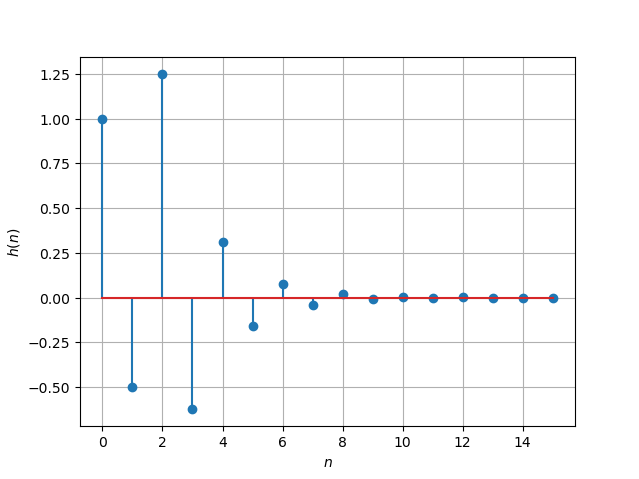
\includegraphics[width=\columnwidth]{figures/Figure_5_3.png}
% 	\end{center}
% 	\captionof{figure}{}
% 	\label{fig:xnyn}	
% \end{figure}
From \eqref{eq:hn_exp} we know that\\
\begin{equation}
	h(n) = \brak{-\frac{1}{2}}^{n}u(n) + \brak{-\frac{1}{2}}^{n-2}u(n-2)
\end{equation}
Implies we can write that\\
\begin{align}
	h\brak{n} &= \begin{cases}
					 0 &, n < 0\\
					 \brak{\frac{-1}{2}}^n &, 0\leq n<2\\
					 5\brak{\frac{-1}{2}}^n &, n \geq 2
				  \end{cases}\label{eq:hn_theoritical_def}
\end{align}
A sequence is said to be bounded when 
\begin{align}
	\abs{x_n} \leq M , \forall n \in \mathcal{N}\label{def:bounded_seq_def}
\end{align}  
Now consider \eqref{eq:hn_theoritical_def},\\
For n$<$0,
\begin{equation}
	\abs{h\brak{n}} \leq 0
\end{equation}
For $0 \leq n <$ 2,
\begin{align}
	\abs{h\brak{n}} = (\frac{1}{2})^n\\
	\implies \abs{h\brak{n}} \leq 1
\end{align}
For $n\geq 2$,
\begin{align}
	\abs{h\brak{n}} = 5(\frac{1}{2})^n\\
	\implies \abs{h\brak{n}} \leq 5
\end{align}
From above we can say that,
      \begin{align}
        M &= max\cbrak{0,1,5} \\
          &= 5\label{eq:hn_bounded_proof}
      \end{align}
Therefore since $M$ exists and is a real value, we can say that h\brak{n} is bounded.

\item Convergent? Justify using the ratio test.
\\
\solution 
\\Yes, it is convergent. We can clearly see in the plot it is not tending to infinite and remain finite.
\\
For large $n$, we see that 
\begin{align}
	h(n) &= \brak{-\frac{1}{2}}^n + \brak{-\frac{1}{2}}^{n - 2} \\
		 &= \brak{-\frac{1}{2}}^{n}\brak{4 + 1} = 5\brak{-\frac{1}{2}}^n \\
		 &\implies \left|\frac{h(n + 1)}{h(n)}\right| = \frac{1}{2}
\end{align}
and therefore, $\lim_{n \to \infty}\left|\frac{h(n + 1)}{h(n)}\right| = \frac{1}{2} < 1$. Hence, we see that $h(n)$ converges.
\\

\item The system with $h(n)$ is defined to be stable if
\begin{equation}
\sum_{n=-\infty}^{\infty}h(n) < \infty
\end{equation}
Is the system defined by \eqref{eq:iir_filter} stable for the impulse response in \eqref{eq:impulse_resp}?
\\
\solution By using h(n) from 5.3
\begin{align}
h(n) &= \brak{-\frac{1}{2}}^{n}u(n) + \brak{-\frac{1}{2}}^{n-2}u(n-2)
\\
&= \sum_{n=-\infty}^{\infty} \brak{-\frac{1}{2}}^{n}u(n) + \brak{-\frac{1}{2}}^{n-2}u(n-2)
\\
&= \sum_{n=-\infty}^{\infty} \brak{-\frac{1}{2}}^{n}u(n) + \sum_{n=-\infty}^{\infty}  \brak{-\frac{1}{2}}^{n-2}u(n-2) 
\\
&= \sum_{n=-\infty}^{\infty} \brak{-\frac{1}{2}}^{n} + \sum_{n=-\infty}^{\infty}  \brak{-\frac{1}{2}}^{n-2}
\\
\\
&= \frac{2}{3} + \frac{2}{3} < \infty 
\\
\\
&= \frac{4}{3} < \infty 
\end{align}
%
\item Verify the above result using a python code.
\\\solution
The following code computes and plots at each n. We can see that the sum converges to a constant value as n tends to infinity.
\lstinputlisting{codes/5_6.py}
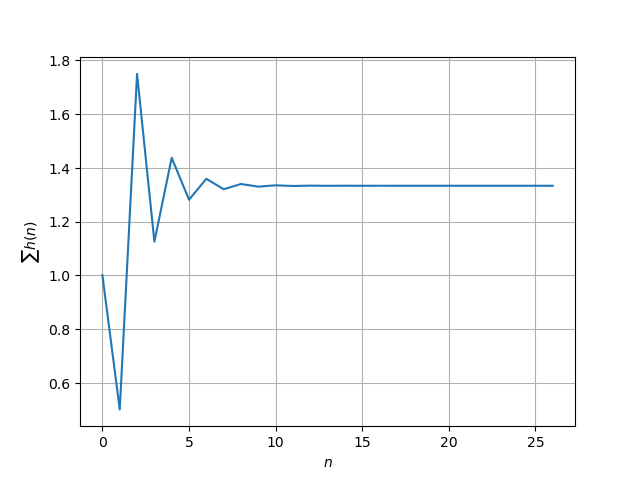
\includegraphics[width=\columnwidth]{figures/Figure_5_6_new.png}
\item 
Compute and sketch $h(n)$ using 
\begin{equation}
\label{eq:iir_filter_h}
h(n) + \frac{1}{2}h(n-1) = \delta(n) + \delta(n-2), 
\end{equation}
%
This is the definition of $h(n)$.
\\
\solution The following code plots Fig. \ref{fig:hndef}. Note that this is the same as Fig. 
\ref{fig:hn}. 
\begin{align}
h(n) + \frac{1}{2}h(n-1) = \delta(n) + \delta(n-2)
\\
H(z) + \frac{1}{2}z^{-1}H(z) = 1+z^{-2}
\\
H(z) = \frac{1}{1 + \frac{1}{2}z^{-1}} + \frac{ z^{-2}}{1 + \frac{1}{2}z^{-1}} , \quad \abs{\frac{1}{2}} < \abs{z}
\\
h(n) = \brak{-\frac{1}{2}}^{n}u(n) + \brak{-\frac{1}{2}}^{n-2}u(n-2)
\end{align}
%
\lstinputlisting{codes/5_3.py}
\begin{figure}[!ht]
\centering
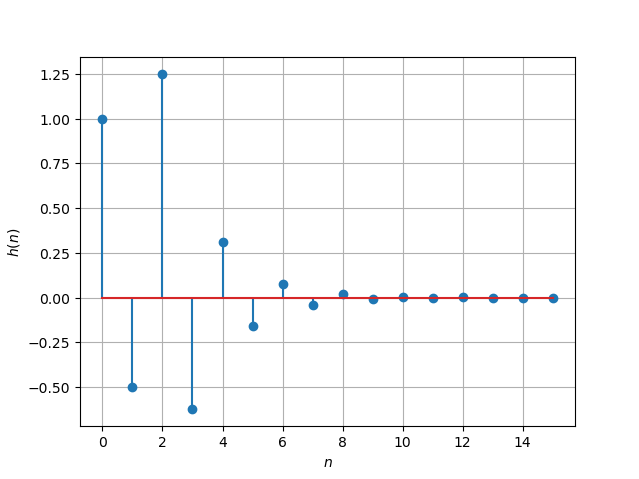
\includegraphics[width=\columnwidth]{figures/Figure_5_3.png}
\caption{$h(n)$ from the definition}
\label{fig:hndef}
\end{figure}
%
\item Compute 
%
\begin{equation}
\label{eq:convolution}
y(n) = x(n)*h(n) = \sum_{n=-\infty}^{\infty}x(k)h(n-k)
\end{equation}
%
Comment. The operation in \eqref{eq:convolution} is known as
{\em convolution}.
%
\\
\solution
The following code plots $y(n)$. 
\lstinputlisting{codes/5_6.py}
\begin{figure}[!ht]
	\centering
	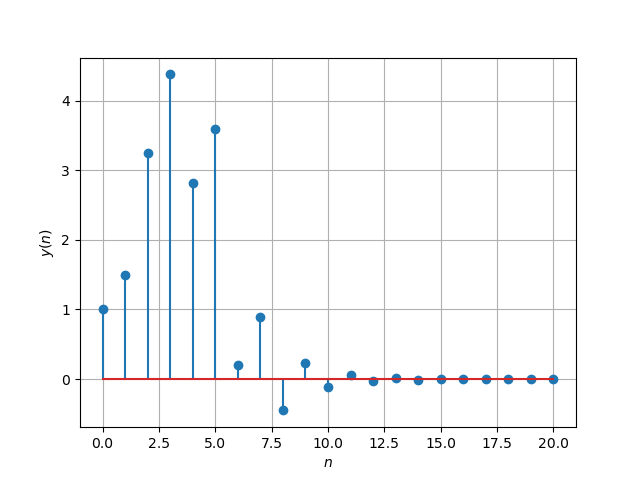
\includegraphics[width=\columnwidth]{figures/Figure_5_6.png}
	\caption{$h(n)$ from the definition}
	\label{fig:hndef}
	\end{figure}
\\
\item Express the above convolution using a Teoplitz matrix.
\\\solution
We know that from, \eqref{eq:convolution},
\begin{equation}
	y(n) = x(n)*h(n) = \sum_{k=-\infty}^{\infty}x(k)h(n-k)
\end{equation}
This can also be wrtten as a matrix-vector multiplication given by the expression,
\begin{equation}
	\label{eq:conv_matrix_vec_mult}
	y = T\brak{h}*x
\end{equation}
In the equation \eqref{eq:conv_matrix_vec_mult}, $T\brak{h}$ is a Teoplitz matrix.
\\ The equation \eqref{eq:conv_matrix_vec_mult} can be expanded as,
\begin{align}
	\mtx{y} &= \mtx{x} \circledast \mtx{h}\\
	\mtx{y} &= 
	\begin{pmatrix}
		h_1 & 0 & . & . & . & 0 \\
		h_2 & h_1 & . & . & . & 0 \\
		h_3 & h_2 & h_1 & . & . & 0 \\
		. & . & . & . & . & . \\
		h_{n-1} & h_{n-2} & h_{n-3} & . & . & 0\\
		h_{n} & h_{n-1} & h_{n-2} & . & . & h_1\\
		0 & h_{n} & h_{n-1} & h_{n-2} & . & h_2\\
		. & . & . & . & . & . \\
		0 & . & . & . & 0 & h_{n-1} \\
		0 & . & . & . & 0 & h_n \\
	\end{pmatrix}
	\begin{pmatrix}
		x_1 \\ x_2 \\ .\\.\\. \\ x_n
	\end{pmatrix}
\end{align}
\item Show that
\begin{equation}
y(n) =  \sum_{n=-\infty}^{\infty}x(n-k)h(k)
\end{equation}
\solution
From \eqref{eq:convolution}, we substitute $k := n - k$ to get
\begin{align}
y\brak{n} &= \sum_{k=-\infty}^{\infty}x\brak{k}h\brak{n - k} \\
		  &= \sum_{n - k=-\infty}^{\infty}x\brak{n - k}h\brak{k} \\
		  &= \sum_{k=-\infty}^{\infty}x\brak{n - k}h\brak{k}
\end{align}
\end{enumerate}
%
\section{DFT and FFT}
\begin{enumerate}[label=\thesection.\arabic*]
\item
Compute
\begin{equation}
X(k) \define \sum _{n=0}^{N-1}x(n) e^{-\j2\pi kn/N}, \quad k = 0,1,\dots, N-1
\end{equation}
and $H(k)$ using $h(n)$.
\\\solution\\
From \ref{def:xn}, we know that ,
\begin{equation}
	x(n) = \cbrak{\underset{\uparrow}{1},2,3,4,2,1}
\end{equation}
%  Let, $e^{-j2\pi k} = \omega$. Then,
% \begin{equation}
% 	X(k) = \sum _{n=0}^{N-1}x(n) \omega^{n/N}
% \end{equation}
Here, let, $\omega=e^{-j2\pi k}$. Then,
\begin{align}
	X(k)=1+2\omega^{\frac{1}{5}}+3\omega^{\frac{2}{5}}+4\omega^{\frac{3}{5}}+2\omega^{\frac{4}{5}}+\omega
	\label{eq:Xkdef}
\end{align}
Similarly, we know from \eqref{eq:hn_theoritical_def},
\begin{align}
	h\brak{n} &= \begin{cases}
					 0 &, n < 0\\
					 \brak{\frac{-1}{2}}^n &, 0\leq n<2\\
					 5\brak{\frac{-1}{2}}^n &, n \geq 2
				  \end{cases}
\end{align}
Now,again let, $\omega=e^{-j2\pi k}$. Then,
\begin{align}
	H(k)=1+\frac{-1}{2}\omega^{\frac{1}{5}}+\frac{5}{4}\omega^{\frac{2}{5}}+\frac{-5}{8}\omega^{\frac{3}{5}}+\frac{5}{16}\omega^{\frac{4}{5}}+\frac{-5}{32}\omega
	\label{eq:Hkdef}
\end{align}
\item Compute 
\begin{equation}
Y(k) = X(k)H(k)
\end{equation}
\\\solution
\\Now, from \eqref{eq:Xkdef} and \eqref{eq:Hkdef}, we know $X(k) and H(k)$. Now, given that,
\begin{equation}
	Y\brak{k}=X\brak{k}*H\brak{k}
\end{equation}
%\polyadd\PolynomX{1+2\omega^{\frac{1}{5}}+3\omega^{\frac{2}{5}}+4\omega^{\frac{3}{5}}+2\omega^{\frac{4}{5}}+\omega}{0}
\begin{multline}
	Y\brak{k}= (1+2\omega^{\frac{1}{5}}+3\omega^{\frac{2}{5}}+4\omega^{\frac{3}{5}}+2\omega^{\frac{4}{5}}+\omega)* \\(1+\frac{-1}{2}\omega^{\frac{1}{5}}+\frac{5}{4}\omega^{\frac{2}{5}}+\frac{-5}{8}\omega^{\frac{3}{5}}+\frac{5}{16}\omega^{\frac{4}{5}}+\frac{-5}{32}\omega)
\end{multline}
\begin{multline}
	Y\brak{k}= 1+\frac{3}{2}\omega^{\frac{1}{5}}+\frac{13}{4}\omega^{\frac{2}{5}}+\frac{35}{8}\omega^{\frac{3}{5}}+\frac{45}{16}\omega^{\frac{4}{5}}\\\frac{115}{32}\omega^{\frac{5}{5}}+\frac{1}{8}\omega^{\frac{6}{5}}+\frac{25}{32}\omega^{\frac{7}{5}}-\frac{5}{8}\omega^{\frac{8}{5}}\\-\frac{5}{32}\omega^{5} 
\end{multline}
where, $\omega=e^{-j2k\pi}$
\item Compute
\begin{equation}
 y\brak{n}={\frac {1}{N}}\sum _{k=0}^{N-1}Y\brak{k}\cdot e^{\j 2\pi kn/N},\quad n = 0,1,\dots, N-1
\end{equation}
\\
\solution The following code plots Fig. \ref{fig:ynconv} and computes $X(k)$
and $Y(k)$. Note that this is the same as 
$y(n)$ in  Fig. \ref{fig:A1_3}. 
%
\lstinputlisting{codes/6_2.py}

\begin{figure}[!ht]
\centering
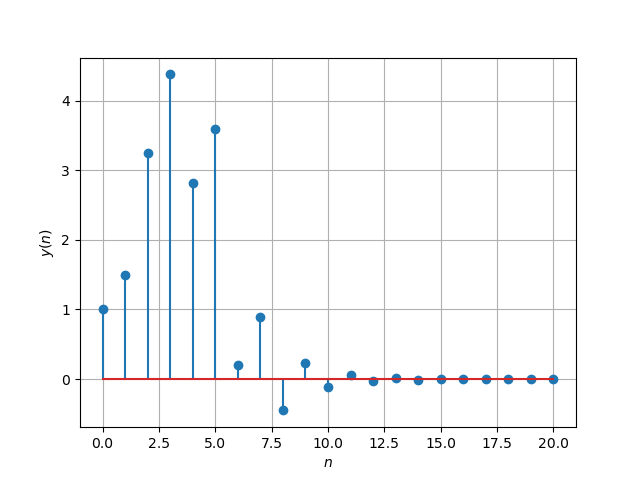
\includegraphics[width=\columnwidth]{figures/Figure_5_6.png}
\caption{$y(n)$ from the DFT}
\label{fig:yndft}
\end{figure}

\item Repeat the previous exercise by computing $X(k), H(k)$ and $y(n)$ through FFT and 
IFFT.
\\
\solution
The following python codes compute $X(k), H(k)$ and $y(n)$ through FFT and 
IFFT.
\lstinputlisting{codes/6_4.py}
\begin{figure}[!ht]
	\centering
	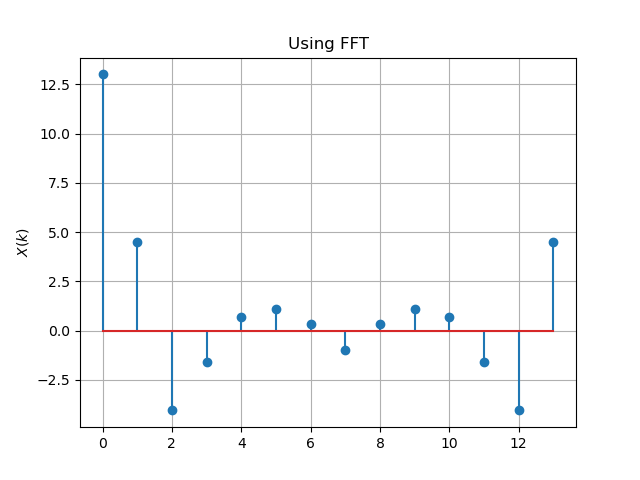
\includegraphics[width=\columnwidth]{figures/Figure_6_4_X.png}
	\caption{$X(k)$ from the FFT}
	% \label{fig:yndft}
\end{figure}
\begin{figure}[!ht]
	\centering
	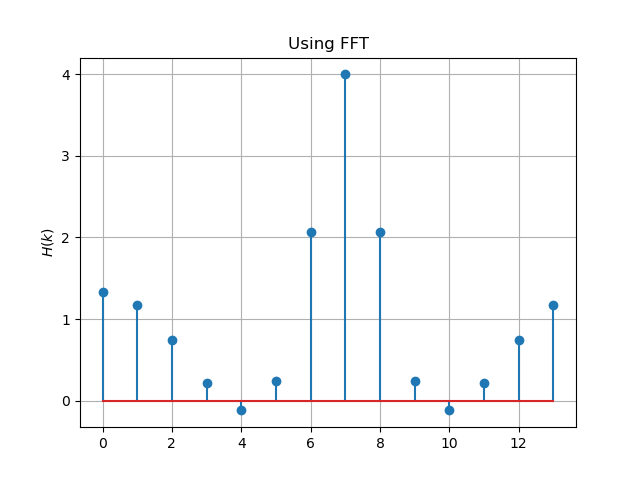
\includegraphics[width=\columnwidth]{figures/Figure_6_4_H.png}
	\caption{$H(k)$ from the FFT}
	% \label{fig:yndft}
\end{figure}
\begin{figure}[!ht]
	\centering
	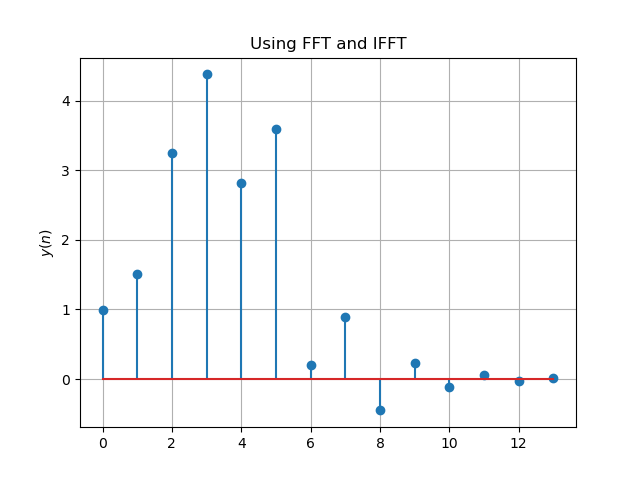
\includegraphics[width=\columnwidth]{figures/Figure_6_4y.png}
	\caption{$y(n)$ from the IFFT}
	% \label{fig:yndft}
\end{figure}
% \item Wherever possible, express all the above equations as matrix equations.
% \end{enumerate}
%
\item Wherever possible, express all the above equations as matrix equations.
\\
\solution
We use the DFT Matrix, where $\omega = e^{-\frac{j2k\pi}{N}}$, which is given by
\begin{align}
	\mtx{W} = 
	\begin{pmatrix}
		\omega^0 & \omega^0 & \ldots & \omega^0 \\
		\omega^0 & \omega^1 & \ldots & \omega^{N - 1} \\
		\vdots & \vdots & \ddots & \vdots \\
		\omega^0 & \omega^{N - 1} & \ldots & \omega^{(N -1)(N - 1)}
	\end{pmatrix}
\end{align}
i.e. $W_{jk} = \omega^{jk}$, $0 \leq j, k < N$. Hence, we can write any DFT equation as
\begin{align}
	\mtx{X} = \mtx{W}\mtx{x} = \mtx{x}\mtx{W}
\end{align}
\noindent where
\begin{align}
	\mtx{x} = 
	\begin{pmatrix}
		x(0) \\ x(1) \\ \vdots \\ x(n - 1)
	\end{pmatrix}
\end{align}
\noindent Using \eqref{eq:inv-ft}, the inverse Fourier Transform is given by
\begin{align}
	\mtx{x} = \mathcal{F}^{-1}\brak{\mtx{X}} = \mtx{W}^{-1}\mtx{X} &= 
	\frac{1}{N}\mtx{W^{H}}\mtx{X} = \frac{1}{N}\mtx{X}\mtx{W^{H}} \\ 
	\implies \mtx{W}^{-1} &= \frac{1}{N}\mtx{W^{H}}
\end{align}
\noindent where $H$ denotes hermitian operator. We can rewrite \eqref{eq:fp} using the
element-wise multiplication operator as
\begin{align}
	\mtx{Y} = \mtx{H}\cdot\mtx{X} = \brak{\mtx{W}\mtx{h}}\cdot\brak{\mtx{W}\mtx{x}}
\end{align}
The plot of $y(n)$ using the DFT matrix in Fig. \eqref{fig:yn-mtx} is the same as $y(n)$ in 
Fig. \eqref{fig:A1_3}. 
\lstinputlisting{codes/6_5_new.py}
%	\end{enumerate}
\begin{figure}[!htb]
	\centering
	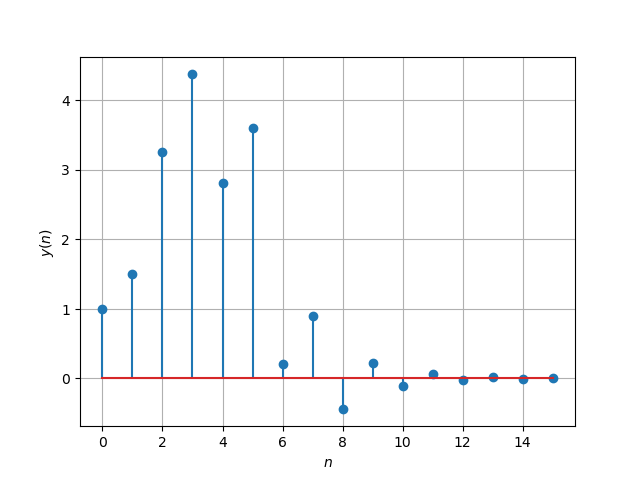
\includegraphics[width=\columnwidth]{figures/Figure_6_5_yn_DFFT.png}
	\caption{$y(n)$ using the DFT matrix}
	\label{fig:yn-mtx}
\end{figure}
% \item Verify the above equations by generating the DFT matrix in python.\\
% \solution
% \begin{figure}[!htb]
% 	\centering
% 	\includegraphics[width=\columnwidth]{./figs/6_6.png}
% 	\caption{$y(n)$ using the DFT matrix}
% 	\label{fig:yn-mtx}
% \end{figure}
%\item Verify the above equations by generating the DFT matrix in python.
\end{enumerate}
%

% \section{FFT}
% % \subsection{Definitions}
% \begin{enumerate}[label=\arabic*.,ref=\thesection.\theenumi]
% \numberwithin{equation}{section}
%     \item The DFT of $x(n)$ is given by
%     \begin{align}
%         X(k) \triangleq \sum_{n=0}^{N-1} x(n) e^{-j 2 \pi k n / N}, \quad k=0,1, \ldots, N-1
%     \end{align}
% \item Let 
% 	\begin{align}
% W_{N} = e^{-j2\pi/N} 
% 	\end{align}
% 		Then the $N$-point {\em DFT matrix} is defined as 
% 	\begin{align}
% 		\vec{F}_{N} = \sbrak{W_{N}^{mn}}, \quad 0 \le m,n \le N-1 
% 	\end{align}
% 	where $W_{N}^{mn}$ are the elements of $\vec{F}_{N}$.
% \item Let 
% 	\begin{align}
% 		\vec{I}_4 = \myvec{\vec{e}_4^{1} &\vec{e}_4^{2} &\vec{e}_4^{3} &\vec{e}_4^{4} }
% 	\end{align}
% 		be the $4\times 4$ identity matrix.  Then the 4 point {\em DFT permutation matrix} is defined as 
% 	\begin{align}
% 		\vec{P}_4 = \myvec{\vec{e}_4^{1} &\vec{e}_4^{3} &\vec{e}_4^{2} &\vec{e}_4^{4} }
% 	\end{align}
% \item The 4 point {\em DFT diagonal matrix} is defined as 
% 	\begin{align}
% 		\vec{D}_4 = diag\myvec{W_{4}^{0} & W_{N}^{1} & W_{N}^{2} & W_{N}^{3}}
% 	\end{align}
% \item Show that 
% \begin{equation}
%     W_{N}^{2}=W_{N/2}
% \end{equation}
% \solution We write
% \begin{align}
% 	W_N^2 = \brak{e^{-\frac{\j2\pi}{N}}}^2 = e^{-\frac{\j2\pi}{N/2}} = W_{N/2}
% \end{align}
% \item Show that 
% \begin{equation}
% 	\vec{F}_{4}=
% \begin{bmatrix}
% 	\vec{I}_{2} & \vec{D}_{2} \\
% \vec{I}_{2} & -\vec{D}_{2}
% \end{bmatrix}
% \begin{bmatrix}
% \vec{F}_{2} & 0 \\
% 0 & \vec{F}_{2}
% \end{bmatrix}
% \vec{P}_{4}
% \end{equation}
% \solution Observe that for $n \in \mathbb{N}$, $W_4^{4n} = 1$ and $W_4^{4n + 2} = -1$. Using \eqref{eq:n-2},
% \begin{align}
% 	\vec{D}_2\vec{F}_2 &= \mybvec{\w{4}{0} & 0 \\ 0 & \w{4}{1}}\mybvec{\w{2}{0} & \w{2}{0} \\ \w{2}{0} & \w{2}{1}} \\
% 					   &= \mybvec{\w{4}{0} & 0 \\ 0 & \w{4}{1}}\mybvec{\w{4}{0} & \w{4}{0} \\ \w{4}{0} & \w{4}{2}} \\
% 					   &= \mybvec{\w{4}{0} & \w{4}{0} \\ \w{4}{1} & \w{4}{3}} \label{eq:fft-df1} \\
% 	\implies -\vec{D}_2\vec{F}_2 &= \mybvec{\w{4}{2} & \w{4}{6} \\ \w{4}{3} & \w{4}{9}} \label{eq:fft-df2}
% \end{align}
% and
% \begin{align}
% 	\vec{F}_2 &= \myvec{\w{2}{0} & \w{2}{0} \\ \w{2}{0} & \w{2}{1}} \\
% 			  &= \myvec{\w{4}{0} & \w{4}{0} \\ \w{4}{0} & \w{4}{2}}
% \end{align}
% Hence,
% \begin{align}
% 	\vec{W}_4 &= \myvec{\w{4}{0} & \w{4}{0} & \w{4}{0} & \w{4}{0} \\
% 		\w{4}{0} & \w{4}{2} & \w{4}{1} & \w{4}{3} \\
% 		\w{4}{0} & \w{4}{4} & \w{4}{2} & \w{4}{6} \\
% 		\w{4}{0} & \w{4}{6} & \w{4}{3} & \w{4}{9} 
% 	} \label{eq:fft-permutation} \\
% 	&= \mybvec{\vec{I}_2\vec{F}_2 & \vec{D}_2{F}_2 \\ \vec{I}_2\vec{F}_2 & -\vec{D}_2{F}_2} \\
% 	&= \mybvec{\vec{I}_2 & \vec{D}_2 \\ \vec{I}_2 & \vec{D}_2}\mybvec{\vec{F}_2 & 0 \\ 0 & \vec{F}_2}
% 	\label{eq:ifd}
% \end{align}
% Multiplying \eqref{eq:ifd} by $\vec{P}_4$ on both sides, and noting that $\vec{W}_4\vec{P}_4 = \vec{F}_4$ gives us.
%% Section 7

\section{FFT}
% \subsection{Definitions}
\begin{enumerate}[label=\arabic*.,ref=\thesection.\theenumi]
\numberwithin{equation}{section}
    \item The DFT of $x(n)$ is given by
    \begin{align}
        X(k) \triangleq \sum_{n=0}^{N-1} x(n) e^{-j 2 \pi k n / N}, \quad k=0,1, \ldots, N-1
    \end{align}
\item Let 
	\begin{align}
W_{N} = e^{-j2\pi/N} 
	\end{align}
		Then the $N$-point {\em DFT matrix} is defined as 
	\begin{align}
		\vec{F}_{N} = \sbrak{W_{N}^{mn}}, \quad 0 \le m,n \le N-1 
	\end{align}
	where $W_{N}^{mn}$ are the elements of $\vec{F}_{N}$.
\item Let 
	\begin{align}
		\vec{I}_4 = \myvec{\vec{e}_4^{1} &\vec{e}_4^{2} &\vec{e}_4^{3} &\vec{e}_4^{4} }
	\end{align}
		be the $4\times 4$ identity matrix.  Then the 4 point {\em DFT permutation matrix} is defined as 
	\begin{align}
		\vec{P}_4 = \myvec{\vec{e}_4^{1} &\vec{e}_4^{3} &\vec{e}_4^{2} &\vec{e}_4^{4} }
	\end{align}
\item The 4 point {\em DFT diagonal matrix} is defined as 
	\begin{align}
		\vec{D}_4 = diag\myvec{W_{4}^{0} & W_{N}^{1} & W_{N}^{2} & W_{N}^{3}}
	\end{align}
\item Show that 
\begin{equation}
    W_{N}^{2}=W_{N/2}
\end{equation}
\solution We write
\begin{align}
	W_N^2 = \brak{e^{-\frac{\j2\pi}{N}}}^2 = e^{-\frac{\j2\pi}{N/2}} = W_{N/2}
\end{align}
%    \item Find $\vec{P}_6$.
%    \item Find $\vec{D}_3$.
    \item Show that 
\begin{equation}
	\vec{F}_{4}=
\begin{bmatrix}
	\vec{I}_{2} & \vec{D}_{2} \\
\vec{I}_{2} & -\vec{D}_{2}
\end{bmatrix}
\begin{bmatrix}
\vec{F}_{2} & 0 \\
0 & \vec{F}_{2}
\end{bmatrix}
\vec{P}_{4}
\end{equation}
\solution Observe that for $n$ in \mathbb{N}$, $W_4^{4n} = 1$ and $W_4^{4n + 2} = -1$. Using \eqref{eq:n-2},
\begin{align}
	\vec{D}_2\vec{F}_2 &= \mybvec{\w{4}{0} & 0 \\ 0 & \w{4}{1}}\mybvec{\w{2}{0} & \w{2}{0} \\ \w{2}{0} & \w{2}{1}} \\
					   &= \mybvec{\w{4}{0} & 0 \\ 0 & \w{4}{1}}\mybvec{\w{4}{0} & \w{4}{0} \\ \w{4}{0} & \w{4}{2}} \\
					   &= \mybvec{\w{4}{0} & \w{4}{0} \\ \w{4}{1} & \w{4}{3}} \label{eq:fft-df1} \\
	\implies -\vec{D}_2\vec{F}_2 &= \mybvec{\w{4}{2} & \w{4}{6} \\ \w{4}{3} & \w{4}{9}} \label{eq:fft-df2}
\end{align}
and
\begin{align}
	\vec{F}_2 &= \myvec{\w{2}{0} & \w{2}{0} \\ \w{2}{0} & \w{2}{1}} \\
			  &= \myvec{\w{4}{0} & \w{4}{0} \\ \w{4}{0} & \w{4}{2}}
\end{align}
Hence,
\begin{align}
	\vec{W}_4 &= \myvec{\w{4}{0} & \w{4}{0} & \w{4}{0} & \w{4}{0} \\
		\w{4}{0} & \w{4}{2} & \w{4}{1} & \w{4}{3} \\
		\w{4}{0} & \w{4}{4} & \w{4}{2} & \w{4}{6} \\
		\w{4}{0} & \w{4}{6} & \w{4}{3} & \w{4}{9} 
	} \label{eq:fft-permutation} \\
	&= \mybvec{\vec{I}_2\vec{F}_2 & \vec{D}_2{F}_2 \\ \vec{I}_2\vec{F}_2 & -\vec{D}_2{F}_2} \\
	&= \mybvec{\vec{I}_2 & \vec{D}_2 \\ \vec{I}_2 & \vec{D}_2}\mybvec{\vec{F}_2 & 0 \\ 0 & \vec{F}_2}
	\label{eq:ifd}
\end{align}
Multiplying \eqref{eq:ifd} by $\vec{P}_4$ on both sides, and noting that $\vec{W}_4\vec{P}_4 = \vec{F}_4$ gives us.
\item Show that 
\begin{equation}
\vec{F}_{N}=
\begin{bmatrix}
\vec{I}_{N/2} & \vec{D}_{N/2} \\
\vec{I}_{N/2} & -\vec{D}_{N/2}
\end{bmatrix}
\begin{bmatrix}
\vec{F}_{N/2} & 0 \\
0 & \vec{F}_{N/2}
\end{bmatrix}
\vec{P}_{N}
\end{equation}
\solution Observe that for even $N$ and letting $\vec{f}_N^i$ denote the $i^{\text{th}}$ column of $\vec{F}_N$, from \eqref{eq:fft-df1} and \eqref{eq:fft-df2},
\begin{align}
	\myvec{\vec{D}_{N/2}\vec{F}_{N/2} \\ -\vec{D}_{N/2}\vec{F}_{N/2}} = \myvec{\vec{f}_N^{2} & \vec{f}_N^{4} & \ldots & \vec{f}_N^{N}}
\end{align}
and
\begin{align}
	\myvec{\vec{I}_{N/2}\vec{F}_{N/2} \\ \vec{I}_{N/2}\vec{F}_{N/2}} = \myvec{\vec{f}_N^{1} & \vec{f}_N^{3} & \ldots & \vec{f}_N^{N - 1}}
\end{align}
Thus,
\begin{align}
	&\mybvec{\vec{I}_2\vec{F}_2 & \vec{D}_2\vec{F}_2 \\ \vec{I}_2\vec{F}_2 & -\vec{D}_2\vec{F}_2} = \mybvec{\vec{I}_{N/2} & \vec{D}_{N/2} \\ \vec{I}_{N/2} & -\vec{D}_{N/2}}\mybvec{\vec{F}_{N/2} & 0 \\ 0 & \vec{F}_{N/2}} \nonumber \\
	&= \myvec{\vec{f}_N^{1} & \ldots & \vec{f}_N^{N - 1} & \vec{f}_N^{2} & \ldots & \vec{f}_N^{N}}
\end{align}
and so,
\begin{align}
	&\mybvec{\vec{I}_{N/2} & \vec{D}_{N/2} \\ \vec{I}_{N/2} & -\vec{D}_{N/2}}\mybvec{\vec{F}_{N/2} & 0 \\ 0 & \vec{F}_{N/2}}\vec{P}_{N} \nonumber \\
	&= \myvec{\vec{f}_N^{1} & \vec{f}_N^{2} & \ldots & \vec{f}_N^{N}} = \vec{F}_N
\end{align}
\item Find 
    \begin{align}
	     \vec{P}_4 \vec{x}
    \end{align}
	\solution We have,
	\begin{align}
		\vec{P}_4\vec{x} = \myvec{\vec{e}_4^1 & \vec{e}_4^3 & \vec{e}_4^2 & \vec{e}_4^4}\myvec{x(0)\\x(1)\\x(2)\\x(3)} = \myvec{x(0)\\x(2)\\x(1)\\x(3)}
		\label{eq:x-permute}
	\end{align}
\item Show that 
    \begin{align}
	    \vec{X} = \vec{F}_N \vec{x}
	    \label{eq:dft-mat-def}
    \end{align}
		where $\vec{x}, \vec{X}$ are the vector representations of $x(n), X(k)$ respectively.
		\\
		\solution Writing the terms of $X$, 
		\begin{align}
			X(0) &= x(0) + x(1) + \ldots + x(N - 1) \\
			X(1) &= x(0) + x(1)e^{-\frac{\j2\pi}{N}} + \ldots + \nonumber \\
				 &+ x(N - 1)e^{-\frac{\j2(N - 1)\pi}{N}} \\
				 &\vdots \nonumber \\
			X(N - 1) &= x(0) + x(1)e^{-\frac{\j2(N - 1)\pi}{N}} + \ldots + \nonumber \\
					 &+ x(N - 1)e^{-\frac{\j2(N - 1)(N - 1)\pi}{N}}	
		\end{align}
		Clearly, the term in the $m^{\text{th}}$ row and $n^{\text{th}}$ column is given by ($0 \leq m \leq N - 1$ and $0 \leq n \leq N - 1$) 
		\begin{align}
			T_{mn} = x(n)e^{-\frac{\j2mn\pi}{N}} 
		\end{align}
		and so, we can represent each of these terms as a matrix product
		\begin{align}
			\vec{X} = \vec{F}_N\vec{x}
		\end{align}
		where $\vec{F}_N = \sbrak{e^{-\frac{-\j2mn\pi}{N}}}_{mn}$ for $0 \leq m \leq N - 1$ and $0 \leq n \leq N - 1$. 
\\
\item Derive the following Step-by-step visualisation  of
8-point FFTs into 4-point FFTs and so on
\begin{equation}
\begin{bmatrix}
X(0) \\ 
X(1) \\ 
X(2) \\ 
X(3)
\end{bmatrix}
=
\begin{bmatrix}
X_{1}(0) \\ 
X_{1}(1)\\ 
X_{1}(2)\\
X_{1}(3)\\
\end{bmatrix}
+
\begin{bmatrix}
W^{0}_{8} & 0 & 0 & 0\\
0 & W^{1}_{8} & 0 & 0\\
0 & 0 & W^{2}_{8} & 0\\
0 & 0 & 0 & W^{3}_{8}
\end{bmatrix}
\begin{bmatrix}
X_{2}(0) \\ 
X_{2}(1) \\ 
X_{2}(2) \\
X_{2}(3)
\end{bmatrix}
\end{equation}
\begin{equation}
\begin{bmatrix}
X(4) \\ 
X(5) \\ 
X(6) \\ 
X(7)
\end{bmatrix}
=
\begin{bmatrix}
X_{1}(0) \\ 
X_{1}(1)\\ 
X_{1}(2)\\
X_{1}(3)\\
\end{bmatrix}
-
\begin{bmatrix}
W^{0}_{8} & 0 & 0 & 0\\
0 & W^{1}_{8} & 0 & 0\\
0 & 0 & W^{2}_{8} & 0\\
0 & 0 & 0 & W^{3}_{8}
\end{bmatrix}
\begin{bmatrix}
X_{2}(0) \\ 
X_{2}(1) \\ 
X_{2}(2) \\
X_{2}(3)
\end{bmatrix}
\end{equation}
4-point FFTs into 2-point FFTs
\begin{equation}
\begin{bmatrix}
X_{1}(0) \\ 
X_{1}(1)\\ 
\end{bmatrix}
=
\begin{bmatrix}
X_{3}(0) \\ 
X_{3}(1)\\ 
\end{bmatrix}
+
\begin{bmatrix}
W^{0}_{4} & 0\\
0 & W^{1}_{4}
\end{bmatrix}
\begin{bmatrix}
X_{4}(0) \\ 
X_{4}(1) \\ 
\end{bmatrix}
\end{equation}
\begin{equation}
\begin{bmatrix}
X_{1}(2) \\ 
X_{1}(3)\\ 
\end{bmatrix}
=
\begin{bmatrix}
X_{3}(0) \\ 
X_{3}(1)\\ 
\end{bmatrix}
-
\begin{bmatrix}
W^{0}_{4} & 0\\
0 & W^{1}_{4}
\end{bmatrix}
\begin{bmatrix}
X_{4}(0) \\ 
X_{4}(1) \\ 
\end{bmatrix}
\end{equation}
\begin{equation}
\begin{bmatrix}
X_{2}(0) \\ 
X_{2}(1)\\ 
\end{bmatrix}
=
\begin{bmatrix}
X_{5}(0) \\ 
X_{5}(1)\\ 
\end{bmatrix}
+
\begin{bmatrix}
W^{0}_{4} & 0\\
0 & W^{1}_{4}
\end{bmatrix}
\begin{bmatrix}
X_{6}(0) \\ 
X_{6}(1) \\ 
\end{bmatrix}
\end{equation}
\begin{equation}
\begin{bmatrix}
X_{2}(2) \\ 
X_{2}(3)\\ 
\end{bmatrix}
=
\begin{bmatrix}
X_{5}(0) \\ 
X_{5}(1)\\ 
\end{bmatrix}
-
\begin{bmatrix}
W^{0}_{4} & 0\\
0 & W^{1}_{4}
\end{bmatrix}
\begin{bmatrix}
X_{6}(0) \\ 
X_{6}(1) \\ 
\end{bmatrix}
\end{equation}
\begin{equation}
P_{8}
\begin{bmatrix}
x(0) \\ 
x(1) \\ 
x(2) \\ 
x(3) \\ 
x(4) \\ 
x(5) \\
x(6) \\
x(7)
\end{bmatrix}
 = 
\begin{bmatrix}
x(0) \\ 
x(2) \\ 
x(4) \\ 
x(6) \\
x(1) \\ 
x(3) \\ 
x(5) \\
x(7)
\end{bmatrix}
\end{equation}
\begin{equation}
P_{4}
\begin{bmatrix}
x(0) \\ 
x(2) \\ 
x(4) \\ 
x(6) \\
\end{bmatrix}
 = 
\begin{bmatrix}
x(0) \\ 
x(4) \\ 
x(2) \\
x(6)
\end{bmatrix}
\end{equation}
\begin{equation}
P_{4}
\begin{bmatrix}
x(1) \\ 
x(3) \\ 
x(5) \\
x(7)
\end{bmatrix}
 = 
\begin{bmatrix}
x(1) \\ 
x(5) \\ 
x(3) \\ 
x(7) \\
\end{bmatrix}
\end{equation}
Therefore,
\begin{equation}
\begin{bmatrix}
X_{3}(0) \\ 
X_{3}(1)\\ 
\end{bmatrix}
= F_{2}
\begin{bmatrix}
x(0) \\ 
x(4) \\ 
\end{bmatrix}
\end{equation}
\begin{equation}
\begin{bmatrix}
X_{4}(0) \\ 
X_{4}(1)\\ 
\end{bmatrix}
= F_{2}
\begin{bmatrix}
x(2) \\ 
x(6) \\ 
\end{bmatrix}
\end{equation}
\begin{equation}
\begin{bmatrix}
X_{5}(0) \\ 
X_{5}(1)\\ 
\end{bmatrix}
= F_{2}
\begin{bmatrix}
x(1) \\ 
x(5) \\ 
\end{bmatrix}
\end{equation}
\begin{equation}
\begin{bmatrix}
X_{6}(0) \\ 
X_{6}(1)\\ 
\end{bmatrix}
= F_{2}
\begin{bmatrix}
x(3) \\ 
x(7) \\ 
\end{bmatrix}
\end{equation}
\solution We write out the values of performing an 8-point FFT on $\vec{x}$ as follows.
\begin{align}
	X(k) &= \sum_{n = 0}^{7}x(n)e^{-\frac{\j2kn\pi}{8}} \\
		 &= \sum_{n = 0}^{3}\brak{x(2n)e^{-\frac{\j2kn\pi}{4}} + e^{-\frac{\j2k\pi}{8}}x(2n + 1)e^{-\frac{\j2kn\pi}{4}}} \\
		 &= X_1(k) + e^{-\frac{\j2k\pi}{4}}X_2(k) 
\end{align}
where $\vec{X}_1$ is the 4-point FFT of the even-numbered terms and $\vec{X}_2$ is the 4-point FFT of the odd numbered terms. Noticing that for $k \geq 4$,
\begin{align}
	X_1(k) &= X_1(k - 4) \\
	e^{-\frac{\j2k\pi}{8}} &= -e^{-\frac{\j2(k - 4)\pi}{8}}
\end{align}
we can now write out $X(k)$ in matrix form as in \eqref{eq:8-low} and \eqref{eq:8-high}. We also need to solve the two 4-point FFT terms so formed.
\begin{align}
	X_1(k) &= \sum_{n = 0}^{3}x_1(n)e^{-\frac{\j2kn\pi}{8}} \\
		 &= \sum_{n = 0}^{1}\brak{x_1(2n)e^{-\frac{\j2kn\pi}{4}} + e^{-\frac{\j2k\pi}{8}}x_2(2n + 1)e^{-\frac{\j2kn\pi}{4}}} \\
		 &= X_3(k) + e^{-\frac{\j2k\pi}{4}}X_4(k) 
\end{align}
using $x_1(n) = x(2n)$ and $x_2(n) = x(2n + 1)$. Thus we can write the 2-point FFTs
\begin{align}
\begin{bmatrix}
X_{3}(0) \\ 
X_{3}(1)\\ 
\end{bmatrix}
= F_{2}
\begin{bmatrix}
x(0) \\ 
x(4) \\ 
\end{bmatrix} \\
\begin{bmatrix}
X_{4}(0) \\ 
X_{4}(1)\\ 
\end{bmatrix}
= F_{2}
\begin{bmatrix}
x(2) \\ 
x(6) \\ 
\end{bmatrix}
\end{align}
Using a similar idea for the terms $X_2$, 
\begin{align}
\begin{bmatrix}
X_{5}(0) \\ 
X_{5}(1)\\ 
\end{bmatrix}
= F_{2}
\begin{bmatrix}
x(1) \\ 
x(5) \\ 
\end{bmatrix} \\
\begin{bmatrix}
X_{6}(0) \\ 
X_{6}(1)\\ 
\end{bmatrix}
= F_{2}
\begin{bmatrix}
x(3) \\ 
x(7) \\ 
\end{bmatrix}
\end{align}
But observe that from \eqref{eq:x-permute},
\begin{align}
	\vec{P}_8\vec{x} &= \myvec{\vec{x}_1\\\vec{x}_2} \\
	\vec{P}_4\vec{x}_1 &= \myvec{\vec{x}_3\\\vec{x}_4} \\ 
	\vec{P}_4\vec{x}_2 &= \myvec{\vec{x}_5\\\vec{x}_6}
\end{align}
where we define $x_3(k) = x(4k)$, $x_4(k) = x(4k + 2)$, $x_5(k) = x(4k + 1)$, and $x_6(k) = x(4k + 3)$ for $k = 0, 1$.
\item For 
    \begin{align}
	    \vec{x} = \myvec{1\\2\\3\\4\\2\\1}
        \label{eq:equation1}
    \end{align}
    compute the DFT  
		using 
	    \eqref{eq:dft-mat-def}\\
\solution Download the Python code from 
\begin{lstlisting}
$ wget https://raw.githubusercontent.com/samar2605/EE3900/master/filter/codes/A1_7_11.py
\end{lstlisting}
%     \item Repeat the above exercise using the FFT
% 	    after zero padding $\vec{x}$.
% %	    \eqref{eq:fft-mat-def}
\item Write a C program to compute the 8-point FFT. \\
\solution The C code for the above two problems can be downloaded from
\begin{lstlisting}
$ wget https://raw.githubusercontent.com/samar2605/EE3900/master/filter/codes/A1_7_13.c
\end{lstlisting}
\end{enumerate}
%
\section{Exercises}
Answer the following questions by looking at the python code in Problem \ref{prob:output}.
\begin{enumerate}[label=\thesection.\arabic*]
\item
The command
\begin{lstlisting}
	output_signal = signal.lfilter(b, a, input_signal)
	\end{lstlisting}
in Problem \ref{prob:output} is executed through the following difference equation
\begin{equation}
\label{eq:iir_filter_gen}
 \sum _{m=0}^{M}a\brak{m}y\brak{n-m}=\sum _{k=0}^{N}b\brak{k}x\brak{n-k}
\end{equation}
%
where the input signal is $x(n)$ and the output signal is $y(n)$ with initial values all 0. Replace
\textbf{signal.filtfilt} with your own routine and verify.
%
\lstinputlisting{codes/8_1.py}
\item Repeat all the exercises in the previous sections for the above $a$ and $b$.
\\
\solution
%\begin{align}
%	\mtx{a} =
%	\begin{pmatrix}
%		4.44 \\ 8.78 \\ -9.93 \\ 6.90 \\ -2.93 \\ 0.70 \\ -0.07
%	\end{pmatrix}
%	\mtx{b} = 
%	\begin{pmatrix}
%		5.02 \times 10^{-5} \\ 3.52 \times 10^{-4} \\ 1.05 \times 10^{-3} \\ 1.76 \times 10^{-3} \\ 1.76 \times 10^{-3} \\ 1.05 \times 10^{-3} \\ 3.52 \times 10^{-4} \\ 5.02 \times 10^{-5} 
%	\end{pmatrix}
%\end{align}
For the given values, the difference equation is
\begin{align}
	&y(n) - \brak{4.44}y(n - 1) + \brak{8.78}y(n - 2) \nonumber \\
	&- \brak{9.93}y(n - 3) + \brak{6.90}y(n - 4) \nonumber \\
	&- \brak{2.93}y(n - 5) \nonumber + \brak{0.70}y(n - 6) \nonumber \\
	&- \brak{0.07}y(n - 7) = \brak{5.02 \times 10^{-5}}x(n) \nonumber \\
	&+ \brak{3.52 \times 10^{-4}}x(n - 1) + \brak{1.05 \times 10^{-3}}x(n - 2) \nonumber \\
	&+ \brak{1.76 \times 10^{-3}}x(n - 3) + \brak{1.76 \times 10^{-3}}x(n - 4) \nonumber \\
	&+ \brak{1.05 \times 10^{-3}}x(n - 5) + \brak{3.52 \times 10^{-4}}x(n - 6) \nonumber \\
	&+ \brak{5.02 \times 10^{-5}}x(n - 7)
\end{align}
From \eqref{eq:iir_filter_gen}, we see that the transfer function can be written as follows
\begin{align}
	H(z) &= \frac{\sum_{k = 0}^{N}b(k)z^{-k}}{\sum_{k = 0}^{M}a(k)z^{-k}} \\
		 &= \sum_{i}\frac{r(i)}{1 - p(i)z^{-1}} + \sum_{j}k(j)z^{-j}
	\label{eq:trans-func}
\end{align}
where $r(i)$, $p(i)$, are called residues and poles respectively of the partial 
fraction expansion of $H(z)$. $k(i)$ are the coefficients of the direct polynomial 
terms that might be left over. We can now take the inverse $z$-transform of
\eqref{eq:trans-func} and get using \eqref{eq:anun},
\begin{align}
	h(n) &= \sum_{i}r(i)[p(i)]^nu(n) + \sum_{j}k(j)\delta(n - j)
	\label{eq:h-n-expr}
\end{align}
Substituting the values,
\begin{align}
	&h(n) = [\brak{2.76}\brak{0.55}^n \nonumber \\ 
	&+ \brak{-1.05-1.84\j}\brak{0.57+0.16\j}^n \nonumber \\
	&+ \brak{-1.05+1.84\j}\brak{0.57-0.16\j}^n \nonumber \\
	&+ \brak{-0.53+0.08\j}\brak{0.63+0.32\j}^n \nonumber \\
	&+ \brak{-0.53-0.08\j}\brak{0.63-0.32\j}^n \nonumber \\
	&+ \brak{0.20+0.004\j}\brak{0.75+0.47\j}^n \nonumber \\
	&+ \brak{0.20-0.004\j}\brak{0.75-0.47\j}^n]u(n) \nonumber \\
	&+ \brak{-6.81 \times 10^{-4}}\delta(n)
\end{align}
The values $r(i)$, $p(i)$, $k(i)$ and thus the impulse response function are computed and plotted at
% \begin{lstlisting}
\lstinputlisting{codes/8_1_new.py}
% \end{lstlisting}
The filter frequency response is plotted at
\lstinputlisting{codes/8_2.py}
Observe that for a series $t_n = r^n$, $\frac{t_{n + 1}}{t_n} = r$.
By the ratio test, $t_n$ converges if $|r| < 1$. We note that
observe that $|p(i)| < 1$ and so, as $h(n)$ is the sum of convergent series,
we see that $h(n)$ converges. From Fig. \eqref{fig:butter-imp}, it is clear
that $h(n)$ is bounded. From \eqref{eq:z_trans},
\begin{align}
	\sum_{n = 0}^{\infty}h(n) = H(1) = 1 < \infty
\end{align}
Therefore, the system is stable. From
$h(n)$ is negligible after $n \geq 64$, and we
can apply a 64-bit FFT to get y(n). The following code uses the DFT matrix
to generate $y(n)$.
\lstinputlisting{codes/8_3.py}
\begin{figure}[!htb]
	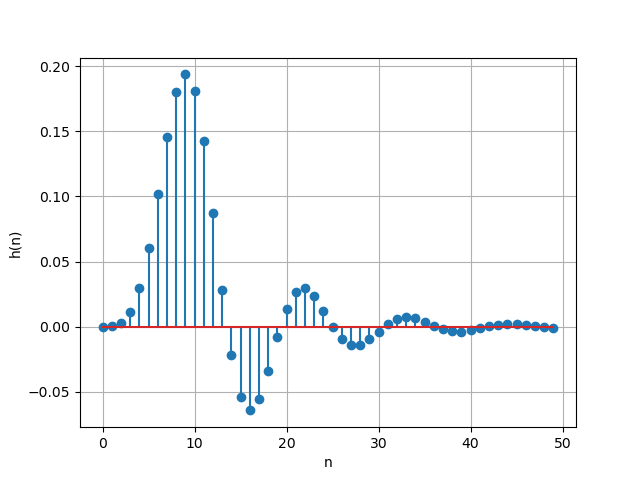
\includegraphics[width=\columnwidth]{figures/Figure_8_1_new.png}
	\caption{Plot of $h(n)$}
	\label{fig:butter-imp}
\end{figure}
\begin{figure}[!htb]
	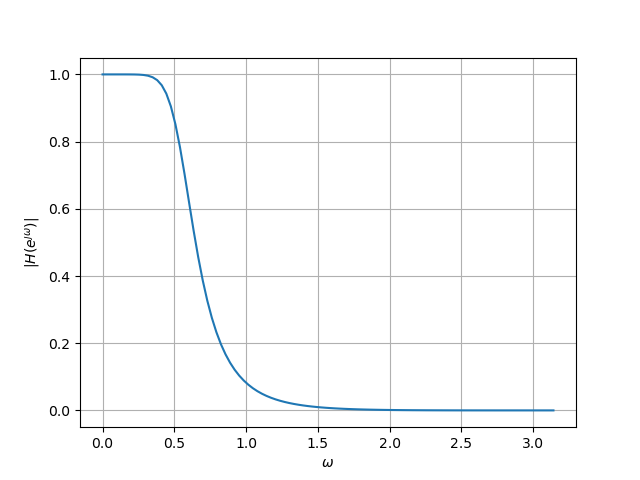
\includegraphics[width=\columnwidth]{figures/Figure_8_2.png}
	\caption{Filter frequency response}
	\label{fig:butter-resp}
\end{figure}
\begin{figure}[!htb]
	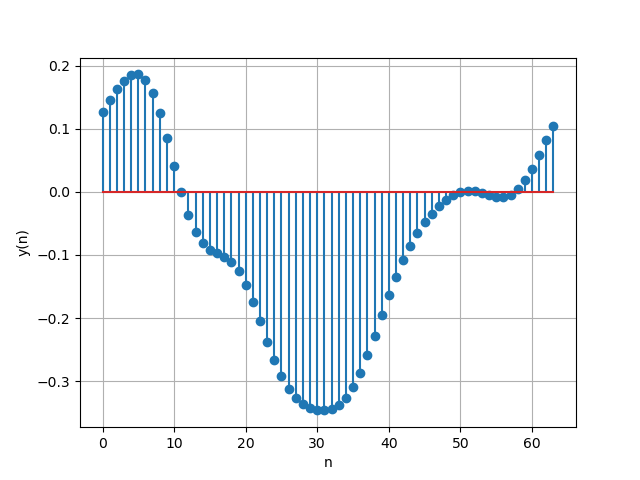
\includegraphics[width=\columnwidth]{figures/Figure_8_3.png}
	\caption{Plot of $y(n)$}
	\label{fig:butter-out}
\end{figure}
\item What is the sampling frequency of the input signal?
\\
\solution
Sampling frequency(fs)=44.1kHZ.
\item
What is type, order and  cutoff-frequency of the above butterworth filter
\\
\solution
The given butterworth filter is low pass with order=2 and cutoff-frequency=4kHz.
%
\item
Modifying the code with different input parameters and to get the best possible output.
%
\solution
A better filtering was found on setting the order of the filter to be 7.
\end{enumerate}
\end{document}